\documentclass[notheorems]{beamer}
\usepackage{SlideStyle}
\renewcommand{\d}{\operatorname{d}}

\titlegraphic{\vspace*{-7cm}
    \parbox[c]{3cm}{
\includegraphics[height=.7cm]{bsulogo}}
    \hspace*{1cm}%
    \parbox[c]{2cm}{
\includegraphics[height=0.6cm]{FPMIlogo_new}}
    \hspace*{1cm}%
    \vspace*{3cm}
}

\title[Модели распространения заболеваний]{\Large ПРОГНОЗИРОВАНИЕ ВРЕМЕННЫХ РЯДОВ НА ОСНОВЕ МОДЕЛЕЙ РАСПРОСТРАНЕНИЯ ЗАБОЛЕВАНИЙ}


\author[В. А. Гут]{Гут Валерия Александровна}

\institute[]{Научный руководитель: С.В. Лобач}


\date[]{}%{\scriptsize \structure{2017-2018}}


\begin{document}

\begin{frame}[plain]
  \titlepage
\end{frame}


%--------------------------------------------------------------------------------------
\begin{frame}{Цели и задачи работы}

\begin{itemize}

\item Объектом исследования является модель SIR (Susceptible-Infectious-Recovered), основанная на разделении населения на три группы.

\item Целью курсовой работы является рассмотрение базовой модели SIR и ее рандомизации.

\end{itemize}

\end{frame}

%--------------------------------------------------------------------------

\begin{frame}
	{Математические модели распространения заболеваний}
	\begin{itemize}
		\item классическая модель SI (Susceptible-Infectious);
		\item базовая модель SIR (Susceptible-Infectious-Recovered);
		\item расширения модели SIR.
	\end{itemize}
\end{frame}

%--------------------------------------------------------------------------

\begin{frame}
	\frametitle{Модель SI}
	Классическая модель SI разбивает предполагает, что все население делится на две группы:
	\begin{itemize}
		\item $S(t)$ = \{люди, подверженные заболеванию (susceptible) в момент времени $t$\};
		\item $I(t)$ = \{инфицированные люди (infectious) в момент времени $t$\}.
	\end{itemize}
	Введем также обозначение $N = \operatorname{const}$ --- общая численность населения.
	
	Ввиду этих обозначений имеет место запись $S(t) + I(t) = N.$
	Скорость изменения числа здоровых и больных людей задается системой ОДУ 
	\begin{eqnarray}
		\left\{ 
		\begin{gathered} 
			\begin{aligned}
				\dfrac{\d S(t)}{\d t} = -\beta\cdot S(t)\cdot I(t),\\
				\dfrac{\d I(t)}{\d t} = \beta\cdot S(t)\cdot I(t),
			\end{aligned}
		\end{gathered} 
		\right.
	\end{eqnarray}
	где $\beta$ -- вероятность заражения здорового человека при контакте с больным.
\end{frame}

%--------------------------------------------------------------------------

\begin{frame}
	\frametitle{Базовая модель SIR}
	Модель SIR основана на разделении населения на три группы: 
	\begin{itemize}
	\item $S(t)$ = \{люди, подверженные заболеванию (susceptible) в момент времени $t$\};
	\item $I(t)$ = \{инфицированные люди (infectious) в момент времени $t$\};
	\item $R(t)$ = \{люди, имеющие иммунитет к болезни (recovered)\}.
	\end{itemize}
	Тогда $S + I + R = N,$ где $N=\operatorname{const}$ -- общая численность населения.
	Модель SIR задается в общем виде системой ОДУ 
	\begin{equation}
		\left\{ 
		\begin{gathered} 
			\begin{aligned}
				\dfrac {\d S(t)}{\d t} &= -\beta \cdot S(t) \cdot I(t),\\
				\dfrac{\d I(t)}{\d t} &= \beta \cdot S(t)\cdot I(t) - \gamma\cdot I(t),\\
				\dfrac{\d R(t)}{\d t} &= \gamma\cdot I(t),
			\end{aligned}
		\end{gathered} 
		\right.
	\end{equation}
	где $\gamma$ -- интенсивность выздоровления.
\end{frame}

%--------------------------------------------------------------------------

\begin{frame}{Модель SIRS}
	 Модель SIRS (Susceptible-Infected-Recovered-Susceptible) является вариацией модели SIR, которая учитывает возможность повторного заражения после выздоровления (потери иммунитета). В модели SIRS существует циклическое движение между состояниями подверженных ($S$), инфицированных ($I$) и восстановленных ($R$). Эта модель задается системой обыкновенных дифференциальных уравнений
	\begin{equation}
		\left\{ 
		\begin{gathered} 
			\begin{aligned}
				\dfrac {\d S(t)}{\d t} &= -\beta \cdot S(t) \cdot I(t) + \lambda \cdot R(t),\\
				\dfrac{\d I(t)}{\d t} &= \beta \cdot S(t)\cdot I(t) - \gamma\cdot I(t),\\
				\dfrac{\d R(t)}{\d t} &= \gamma\cdot I(t) - \lambda \cdot R(t),
			\end{aligned}
		\end{gathered} 
		\right.
	\end{equation}
	где число $\lambda$ определяет вероятность потери иммунитета и перехода из группы $R(t)$ в группу $I(t)$.
\end{frame}

%--------------------------------------------------------------------------

\begin{frame}
	{SEIR-модель}
	В SEIR модели предполагается, что инфекция имеет инкубационный (exposed) период, в течение которого люди инфицированы, но
	еще не заразны. Эта группа людей обозначается через $E(t)$. С учетом нового класса получаем следующую структуру
	популяции:
	$S + E + I + R = N = \operatorname{const}.$
	
	Модель SEIR задается в общем виде системой ОДУ
	\begin{equation}
		\left\{ 
		\begin{gathered} 
			\begin{aligned}
				\dfrac {\d S(t)}{\d t} &= - \beta \cdot I(t)\cdot S(t),\\
				\dfrac {\d E(t)}{\d t} &= \beta \cdot S(t)\cdot I(t) - \sigma\cdot E(t),\\
				\dfrac{\d I(t)}{\d t} &=\sigma \cdot E(t) - \gamma\cdot I(t),\\
				\dfrac{\d R(t)}{\d t} &= \gamma\cdot I(t). 
			\end{aligned}
		\end{gathered} 
		\right.
	\end{equation}
	параметр $\sigma^{-1}$ представляет собой среднюю продолжительность инкубационного периода.
\end{frame}

%--------------------------------------------------------------------------

\begin{frame}
	{Модели SIR с учетом смертности и рождаемости}
	Пусть $\lambda > 0$ и $\mu > 0$ коэффициенты рождаемости и смертности популяции соответственно. Система ОДУ для SIR-модели в предположении, что все рожденные являются здоровыми людьми, имеет вид 
	\begin{equation}
		\left\{ 
		\begin{gathered} 
			\begin{aligned}
				\dfrac {\d S(t)}{\d t} &= -\beta \cdot S(t) \cdot I(t) + \lambda\cdot N(t) - \mu\cdot S(t),\\
				\dfrac{\d I(t)}{\d t} &= \beta \cdot S(t)\cdot I(t) - \gamma\cdot I(t) - \mu\cdot I(t),\\
				\dfrac{\d R(t)}{\d t} &= \gamma\cdot I(t) - \mu \cdot R(t),
			\end{aligned}
		\end{gathered} 
		\right.
	\end{equation}
	где $S(t) + I(t) + R(t) = N(t).$
	
	Складывая все уравнения системы, мы получаем уравнение Мальтуса для численности популяции 
	\begin{equation}
		\dfrac{\d N(t)}{\d t} = (\lambda-\mu) \cdot N(t).
	\end{equation}
\end{frame}

%--------------------------------------------------------------------------

\begin{frame}{Модель MSIR}
		Модель MSIR (M -- «maternally derived immunity») включает класс $M(t)$ (для материнского иммунитета) в начало модели. Модель MSIR с учетом смертности и рождаемости описывается следующими дифференциальными уравнениями:
	\begin{equation}
		\left\{ 
		\begin{gathered} 
			\begin{aligned}
				\dfrac {\d M(t)}{\d t} &= \lambda\cdot N(t) - \delta\cdot M(t)-\mu\cdot M(t),\\
				\dfrac {\d S(t)}{\d t} &= \delta \cdot M(t) -\beta\cdot S(t)\cdot I(t) - \mu \cdot S(t),\\
				\dfrac{\d I(t)}{\d t} &=\beta\cdot S(t)\cdot I(t) - \gamma \cdot S(t) - \mu \cdot I(t),\\
				\dfrac{\d R(t)}{\d t} &= \gamma\cdot I(t) - \mu \cdot R(t), 
			\end{aligned}
		\end{gathered} 
		\right.
	\end{equation}
	где $S(t) + I(t) + R(t) + M(t) = N(t).$
\end{frame}

%--------------------------------------------------------------------------

\begin{frame}
	{Модель MSEIR}
	Модель MSEIR ($M$ -- наделенные иммунитетом от рождения, $S$ -- восприимчивые, $E$ -- контактные, $I$ -- инфицированные, $R$ -- выздоровевшие) -- одна из самых сложных для анализа в силу наличия большого числа независимых параметров. Система уравнений для нее имеет вид:
	\begin{equation}
		\left\{ 
		\begin{gathered} 
			\begin{aligned}
				\dfrac {\d M(t)}{\d t} &= \lambda\cdot N(t) - \delta\cdot M(t)-\mu\cdot M(t),\\
				\dfrac {\d S(t)}{\d t} &= \delta \cdot M(t) -\beta\cdot S(t)\cdot I(t) - \mu \cdot S(t),\\
				\dfrac {\d E(t)}{\d t} &= \beta \cdot S(t)\cdot I(t) - (\sigma + \mu)\cdot E(t),\\
				\dfrac{\d I(t)}{\d t} &=\sigma \cdot E(t) - (\gamma + \mu)\cdot I(t),\\
				\dfrac{\d R(t)}{\d t} &= \gamma\cdot I(t) - \mu \cdot R(t). 
			\end{aligned}
		\end{gathered} 
		\right.
	\end{equation}
	где $M (t)$ -- численность индивидов с приобретенным внутриутробно иммунитетом.
\end{frame}

%--------------------------------------------------------------------------

\begin{frame}
	{Рандомизация базовой SIR модели}
	Произведем обобщение базовой SIR-модели, добавив к ней рандомизацию.
	\begin{equation}
		\left\{ 
		\begin{gathered} 
			\begin{aligned}
				\dfrac {\d S(t)}{\d t} &= -\Big(\beta +\sigma_1 \cdot dW(t)\Big)\cdot S(t)\cdot I(t) ,\\
				\dfrac{\d I(t)}{\d t} &= \Big(\beta +\sigma_1 \cdot dW(t)\Big) \cdot S(t)\cdot I(t) - \Big(\gamma + \sigma_2d W(t)\Big)\cdot I(t),\\
				\dfrac{\d R(t)}{\d t} &= \Big(\gamma + \sigma_2d W(t)\Big)\cdot I(t),
			\end{aligned}
		\end{gathered} 
		\right.		
	\end{equation}
	где $dW (t)$ – производная стохастического винеровского процесса, введенная
	в систему дифференциальных уравнений исходя из предположения, что внешние
	случайные возмущения представляют собой белый шум; $\sigma_1, \sigma_2$ -- это константы, описывающие интенсивность стохастического окружения для процессов инфицирования
	и выздоровления соответственно. 
\end{frame}

%--------------------------------------------------------------------------

\begin{frame}
	{Приближенное численное решение задачи Коши для базовой модели SIR}
	\begin{figure}[h]
		\centering
		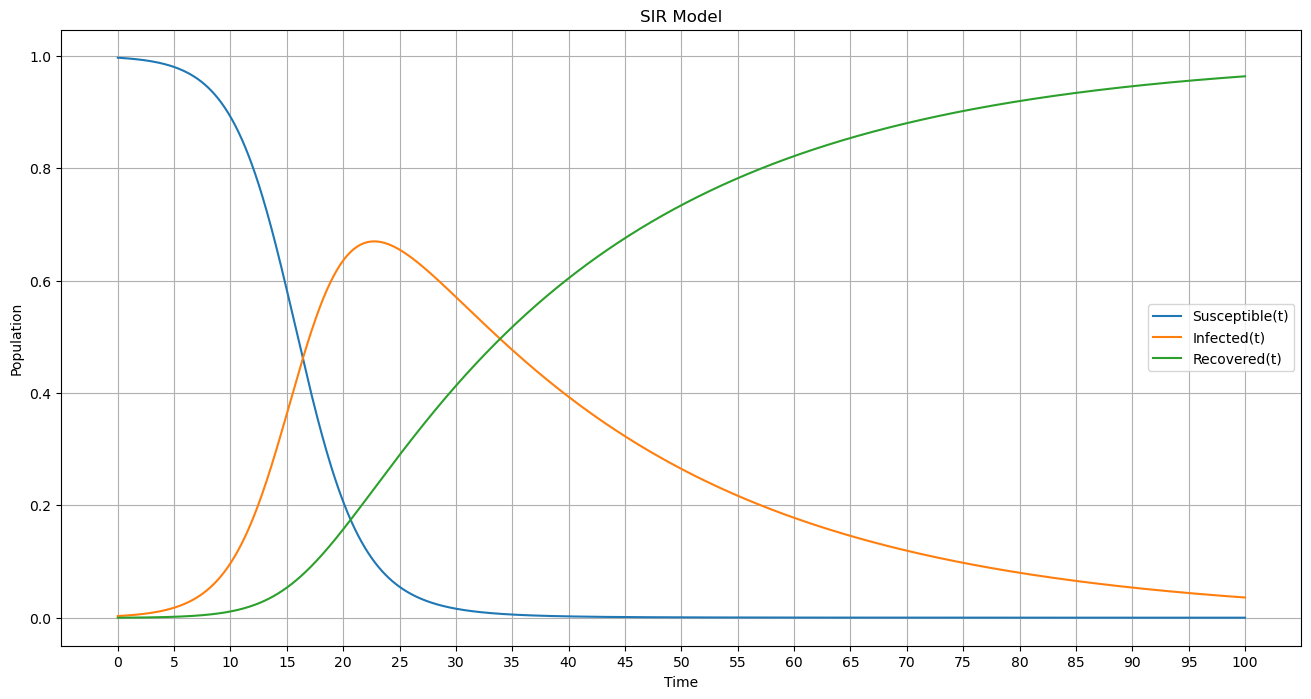
\includegraphics[scale=0.3]{images/img01}
		\caption{Зависимость $S, I, R$ от времени при начальных условиях $S(0) = 997$, $I(0) = 3$, $R(0) = 0$
			интенсивности инфицирования $\beta = 0.4$ и интенсивности выздоровления $\gamma = 0.04$}
		\label{fig:img01}
	\end{figure}
\end{frame}

%--------------------------------------------------------------------------

\begin{frame}
	{Приближенное численное решение задачи Коши для рандомизированной модели SIR}
	\begin{figure}[h]
		\centering
		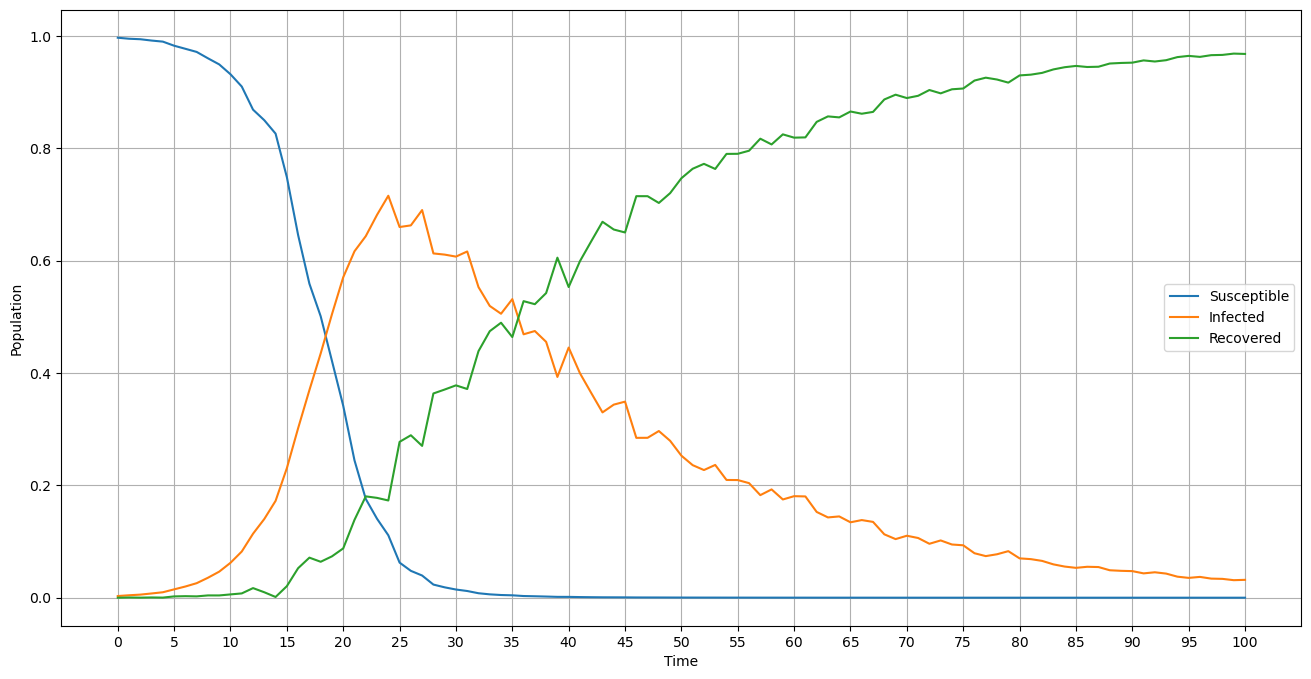
\includegraphics[scale=0.3]{images/img04}
		\caption{Зависимость $S, I, R$ от времени при начальных условиях $S(0) = 997$, $I(0) = 3$, $R(0) = 0$
			интенсивности инфицирования $\beta = 0.4$ и интенсивности выздоровления $\gamma = 0.04$ при $\sigma_1 = 0.1$, $\sigma_2 = 0.05$}
		\label{fig:img04}
	\end{figure}
\end{frame}

%--------------------------------------------------------------------------

\begin{frame}
	{Заключение}
	Основными результатами работы являются построение, исследование базовой и рандомизированной моделей SIR для распространения заболеваний. 
\end{frame}

%--------------------------------------------------------------------------

\begin{frame}
	{Список используемых источников}
	\begin{enumerate}
		\item Statistical forecasting of the dynamics of epidemiological indicators for COVID-19 incidence in the Republic of Belarus / Yu. S. Kharin, V. A. Valoshka, O. V. Dernakova, V. I. Malugin, A. Yu. Kharin// Journal of the Belarusian State University. Mathematics and Informatics. - 2020. - № 3. - С. 36-50
		\item Methods of intellectual data analysis in COVID-19 research / O. V. Senko, A. V. Kuznetsova, E. M. Voronin, O. A. Kravtsova, L. R. Borisova, I. L. Kirilyuk, V. G. Akimkin// Journal of the Belarusian State University. Mathematics and Informatics. – 2022. – № 1. – С. 83-96
		\item Детерминированные и стохастические модели распространения инфекции и тестирование в изолированном контингенте/ Чигарев, А. В.,Журавков, М. А.,Чигарев, В. А.// Журнал Белорусского государственного университета. Математика. Информатика - 2021. - № 3. - С. 57-67
	\end{enumerate}
\end{frame}

%--------------------------------------------------------------------------

\end{document} 